\documentclass[punct]{ctexbeamer}
\usefonttheme{professionalfonts}   % 数学公式字体

\titlegraphic{
\includegraphics[width=2cm]{tjnu.jpg}}

\usepackage{color}
%\lineskip=9pt
\linespread{1.3}\selectfont
\makeatletter
\renewcommand\normalsize{%
	\@setfontsize\normalsize\@xpt\@xiipt
	\abovedisplayskip 3\p@ \@plus3\p@ \@minus3\p@
	\abovedisplayshortskip \z@ \@plus3\p@
	\belowdisplayshortskip 3\p@ \@plus3\p@ \@minus1\p@
	\belowdisplayskip \abovedisplayskip
	\let\@listi\@listI}
\makeatother
\parskip=6pt
%\usepackage{ctex}
%\usepackage[UTF8, heading = false, scheme = plain]{ctex}
%%%=== theme ===%%%
\usetheme{Madrid}
\useinnertheme{circles}
\setbeamertemplate{navigation symbols}{}
%\setbeamertemplate{footline}[page number]
\setbeamertemplate{footline}[frame number]{}
\usepackage{lmodern}
\usepackage{amsmath}
\usepackage{amssymb}
\usepackage{latexsym}
\usepackage{amsthm}
\usepackage{mathrsfs}
\usepackage{tikz}




\setbeamertemplate{theorems}[numbered]
\newtheorem{thm}{定理}
%\newtheorem{thm}{定理}[section]
\newtheorem{prop}[thm]{命题}
\newtheorem{cor}[thm]{推论}
\newtheorem{defi}[thm]{定义}
\newtheorem{lem}[thm]{引理}

\newtheorem{quest}[thm]{问题}
\newtheorem{conj}[thm]{猜想}
\newtheorem{ex}{例}[section]
\newtheorem{pr}{性质}

\newcommand{\blue}{\textcolor{blue}}
\def\pf{\noindent {\bf 证明\ }}
\def\sol{\noindent {\bf 解\ }}


\def\multiset#1#2{\ensuremath{\left(\kern-.3em\left(\genfrac{}{}{0pt}{}{#1}{#2}\right)\kern-.3em\right)}}



\begin{document}

	\title{组\ 合\ 数\ 学}

	\author{张\ 彪}
	\institute[数学科学学院]{\normalsize 天津师范大学}
	%\date[2011年10月13日]{\small 2011年10月13日}
	\date[]{zhang@tjnu.edu.cn}
	\frame[plain]{\titlepage}
%	\begin{frame}
%		\tableofcontents
%	\end{frame}
	\AtBeginSection[]
	{
		\begin{frame}
			\frametitle{Outline}
			\tableofcontents[currentsection]
		\end{frame}
	}
%\section{Fibonacci数列引入}

\begin{frame}
	Fibonacci数列,是由13世纪的意大利数学家Fibonacci提出的,当时是和兔子的繁殖问题有关的。这个问题是:
	\begin{ex}
%		有小兔一对,若第二个月它们成年,第三个月生下小兔一对,以后每月生产一对小兔,而所生小兔亦在第二个月成年,第三个月生产另一对小兔,以后亦每月生产小兔一对,假定每产一对小兔必为一雌一雄,且均无死亡,试问一年后共有兔子几对?
   假定一对刚出生的小兔一个月后就 能长成大兔, 再过一个月便能生下一对小兔, 并且此后每个月都生一对小兔. 假定每产一对小兔必为一雌一雄,且不考虑死亡问 题, 则一对刚出生的兔子, 一年内能繁殖成多少对兔子?
	\end{ex}
\pause
我们用$f(n)$表示第$n$个月兔子对数,则
\begin{table}
	\begin{tabular}{c|ccccccc}
		月份&1&2&3&4&5&6&7\\ \hline
		大兔子&1	&1	&2	&3	&5	&8	&13\\
		小兔子&0&1	&1	&2	&3	&5	&8
	\end{tabular}
\end{table}

\end{frame}

\begin{frame}
	于是
	\begin{table}
		\begin{tabular}{c|ccccccc}
			$n$&1&2&3&4&5&6&7\\ \hline
			$f(n)$&1	&2	&3	&5	&8	&13&21\\

		\end{tabular}
	\end{table}
注意到\[
f(n)=f(n-1)+f(n-2),
\]其中$f(n-1)$表示大兔子的对数,$f(n-2)$表示小兔子的对数。
\end{frame}


\begin{frame}
	\begin{ex}
		用多米诺骨牌($2\times 1$长方块)完全覆盖$n\times 2$棋盘的覆盖方案数。
	\end{ex}
\pause \begin{figure}[h]
	\centering
	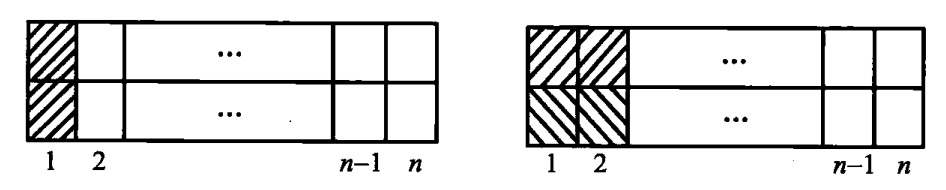
\includegraphics[width=0.8\linewidth]{domino.jpg}
	\caption{ $n\times 2$棋盘覆盖方案}
\end{figure}
\begin{itemize}
	\item 若第一张骨牌覆盖第一列两个方格,则剩下的是$(n-1)\times 2$棋盘的覆盖问题;
	\item 若第一张骨牌覆盖第一行两个方格,则还需一张骨牌覆盖第二行两个方格,剩下的是$(n-2)\times 2$棋盘的覆盖问题。
\end{itemize}
用$f(n)$表示$n\times 2$棋盘的覆盖问题,则有\[
f(n)=f(n-1)+f(n-2).
\]
\end{frame}


\begin{frame}
    \begin{ex}
        一个小孩上楼梯,每次可上一阶或二阶,问上$n$阶楼梯有多少种方案?
    \end{ex}
    \pause
    \begin{table}
        \begin{tabular}{c|c|lllll}
            $n$&方法数&\multicolumn{5}{c}{方案}\\\hline
            1&1	&1	&	&	&	&		\\
            2&2	&1+1	&2	&	&	& \\
            3&3	&1+1+1	&1+2	&2+1	&	&		\\
            4&5	&1+1+1+1	&1+2+1	&1+1+2	&2+1+1	&2+2
        \end{tabular}
    \end{table}
    按最后一步所走楼梯的阶数(1或者2)分类,利用加法规则,得
    \[
    f(n)=f(n-1)+f(n-2),
    \]其中$f(n-1)$表示最后一步上了一阶楼梯的方案数,$f(n-2)$表示最后一阶上了两阶楼梯的方案数。
\end{frame}

%
%
%\section{用生成函数求解Fibonacci数通项表达式}
%\begin{frame}{普通生成函数}
%	设递推关系为\[F_{n}=F_{n-1}+F_{n-2}.\]
%	等式两边同乘以$x^{n}$并关于$n\geq 2$求和得
%	$$
%	\sum_{n \geq 2} F_{n} x^{n}=\sum_{n \geq 2}\left(F_{n-1}+F_{n-2}\right) x^{n} .
%	$$
%
%	令$f(x)=\sum_{n \geq 0} F_{n} x^{n}$ 得
%	$$
%	\sum_{n \geq 2} F_{n} x^{n}=f(x)-F_{0}-F_{1} x=f(x)-x
%	$$
%	且
%	$$
%	\sum_{n \geq 2}\left(F_{n-1}+F_{n-2}\right) x^{n}=x\left(f(x)-F_{0}\right)+x^{2} f(x)=\left(x+x^{2}\right) f(x) .
%	$$
%	令左右两边的表达式相等并求解$f(x)$得到
%	$$
%	f(x)=\frac{x}{1-x-x^{2}} .
%	$$
%
%\end{frame}
%\begin{frame}
%利用部分分式分解
%	$$
%	f(x)=\frac{x}{\left(1-\frac{x}{r_{1}}\right)\left(1-\frac{x}{r_{2}}\right)}=\frac{A}{\left(1-\frac{x}{r_{1}}\right)}+\frac{B}{\left(1-\frac{x}{r_{2}}\right)}.
%	$$
%	$A, B$为常数,$
%	r_{1}=\frac{-1+\sqrt{5}}{2} \quad \text {且} \quad r_{2}=\frac{-1-\sqrt{5}}{2}.
%	$ 约分得
%	$$
%	x=A\left(1-\frac{x}{r_{2}}\right)+B\left(1-\frac{x}{r_{1}}\right) \text {. }
%	$$
%	将 $x=r_{1}$代入此等式化简得  $r_{1}=A\left(1-r_{1} / r_{2}\right)$ , 解出 $A$ 得 $A=1 / \sqrt{5}$. 类似地, 将  $x=r_{2}$ 代入得 $B=-1 / \sqrt{5}$.于是
%	$$
%	f(x)=\frac{1}{\sqrt{5}} \cdot \sum_{n \geq 0} \frac{x^{n}}{r_{1}^{n}}-\frac{1}{\sqrt{5}} \cdot \sum_{n \geq 0} \frac{x^{n}}{r_{2}^{n}}.
%	$$通过分母有理化可以检验 $1 / r_{1}=(1+\sqrt{5}) / 2$ 且 $1 / r_{2}=$ $(1-\sqrt{5}) / 2$. 取两边 $x^{n}$系数得
%	\[
%	F_{n}=\frac{1}{\sqrt{5}}\left(\frac{1+\sqrt{5}}{2}\right)^{n}-\frac{1}{\sqrt{5}}\left(\frac{1-\sqrt{5}}{2}\right)^{n}
%	\]
%\end{frame}
%
%\begin{frame}{指数型生成函数}
%	考虑递推关系\[F_{n+2}=F_{n+1}+F_{n}.\quad(n\geq0)\]
%	令$f(x)=\sum_{n=0}^{\infty}F_{n}\frac{x^{n}}{n!}$,则
%	\[\begin{aligned}
%		f^{\prime}=&\sum_{n=1}{\infty}\frac{nF_{n}x^{n-1}}{n!}\\
%		=&\sum_{n=1}^{\infty}\frac{F_{n}x^{n-1}}{(n-1)!}\\
%		=&\sum_{n=0}^{\infty}F_{n+1}\frac{x^{n}}{n!}
%	\end{aligned}
%	\]类似地,\[f^{\prime\prime}=\sum_{n=0}^{\infty}F_{n+2}\frac{x^{n}}{n!}.\]对递推关系两边同时乘以$\frac{x^{n}}{n!}$并关于$n\geq0$求和得\[
%	f^{\prime\prime}=f^{\prime}+f.
%	\]
%\end{frame}
%
%\begin{frame}
%	上式是一个微分方程,利用解特征根得其通解为
%	\[
%	f(x)=c_{1}e^{r_{1}x}+c_{2}e^{r_{2}x}
%	\]其中$
%	r_{1}=\frac{-1+\sqrt{5}}{2} \quad \text {且} \quad r_{2}=\frac{-1-\sqrt{5}}{2}.
%	$
%
%	代入初值条件$f(0)=0$及$f^{\prime}(0)=1$解得$$c_{1}=\frac{1}{\sqrt{5}},c_{2}=-\frac{1}{\sqrt{5}}.$$于是
%	\[f=\frac{1}{\sqrt{5}}(e^{r_{1}x}-e^{r_{2}x}).\]考虑上式右端$\frac{x^{n}}{n!}$项系数即得$F_{n}$表达式。
%\end{frame}
%

\end{document}